\documentclass[11pt]{amsart}
\usepackage{amsmath,amssymb,amsthm,mathtools}
\usepackage[margin=1in]{geometry}
\usepackage{graphicx}
\usepackage[hidelinks]{hyperref}

\newtheorem{theorem}{Theorem}[section]
\newtheorem{proposition}[theorem]{Proposition}
\newtheorem{definition}[theorem]{Definition}
\theoremstyle{remark}
\newtheorem*{remark}{Remark}

\title{Totient Hyperbolas and the $V_4\leftrightarrow QR(12)$ Bijection\\
\large A companion note to Paper A}
\author{Jeremy Ebert}
\address{Franklin County, Ohio, USA}
\date{2026}

\begin{document}

\begin{abstract}
Paper A \cite{Ebert2026Table} classifies the conic sections cut from the
factor cone $X^2+Y^2=T^2$ by lines $ax+by=c$ in factor coordinates.  For
the units $r\in U(12)=\{1,5,7,11\}$, the sections $X=(r-1)/2$ are
hyperbolas passing through the unit-shell points
$(\pm(r-1)/2,\pm\sqrt r,(r+1)/2)$.  Their vertices
$X\in\{0,2,3,5\}$ and their landing-circle radii
$T\in\{1,3,4,6\}$ square to $QR(12)=\{0,1,4,9\}$ modulo $12$, giving two
bijections $U(12)\to QR(12)$.  The two bijections are complementary,
$\varphi_++\varphi_-\equiv 1\pmod{12}$, and both preserve the genus
bipartition $\{1,11\}\mapsto\{0,1\}$, $\{5,7\}\mapsto\{4,9\}$.  This note
records the construction and its exact scope.
\end{abstract}

\maketitle

\section{Paper-A sections}

We use Paper A's two-sided lift
\[
X=\frac{x-y}{2},\qquad Y=\pm\sqrt{xy},\qquad
T=\frac{x+y}{2},\qquad X^2+Y^2=T^2.
\]
A line $ax+by=c$ with $ab<0$ and $c\ne0$ cuts a nondegenerate hyperbola;
for $c=0$ the section degenerates to the generator pair
\cite{Ebert2026Table}.  The lines
\[
x-y=2c,\qquad\text{i.e. }a=1,\ b=-1,
\]
give the vertical planes $X=c$, whose sections are
\[
T^2-Y^2=c^2,
\]
hyperbolas opening along $T$ (degenerate for $c=0$).

\section{The unit shell}

The units modulo $12$ are
\[
U(12)=\{1,5,7,11\},
\]
and since every element squares to $1\bmod 12$,
\[
U(12)\cong V_4,
\]
the Klein four-group.  The factor pairs $(r,1)$ and $(1,r)$ lift to the
unit-shell points
\begin{equation}\label{eq:shell}
T_r=\frac{r+1}{2},\qquad
X_r=\pm\frac{r-1}{2},\qquad
Y_r=\pm\sqrt r,
\end{equation}
so the four labels occupy the heights
\[
T\in\{1,3,4,6\}.
\]

\section{The four totient hyperbolas}

\begin{definition}
For $r\in U(12)$, the \emph{totient hyperbola} $H_r$ is the Paper-A
section $X=(r-1)/2$ (the $+$ branch; the $-$ branch is its image under
factor exchange $(x,y)\leftrightarrow(y,x)$).
\end{definition}

\begin{proposition}\label{prop:hyperbola}
On the cone, $H_r$ is the hyperbola
\[
T^2-Y^2=\left(\frac{r-1}{2}\right)^2,
\]
nondegenerate for $r>1$ and the degenerate generator pair $T=\pm Y$
for $r=1$.  It contains the shell points
$\bigl(\pm(r-1)/2,\pm\sqrt r,(r+1)/2\bigr)$.
\end{proposition}
\begin{proof}
Intersecting $X=(r-1)/2$ with $X^2+Y^2=T^2$ gives the displayed
equation directly.  At $T=(r+1)/2$,
\[
Y^2=\left(\frac{r+1}{2}\right)^2-\left(\frac{r-1}{2}\right)^2=r,
\]
so the shell points \eqref{eq:shell} lie on $H_r$.
\end{proof}

Figure~\ref{fig:hyperbolas} shows the four hyperbolas.  Each colored arc
is drawn from its vertex (open circle) to its shell points (squares):
the vertex is where $\varphi_-$ is read off, the landing circle where
$\varphi_+$ is read off.

\section{The double $V_4\leftrightarrow QR(12)$ bijection}

The quadratic residues modulo $12$ are
\[
QR(12)=\{0,1,4,9\}.
\]
Each totient hyperbola determines two canonical integers: its vertex
$X=(r-1)/2$ (closest approach to the $T$-axis) and its landing-circle
radius $T=(r+1)/2$ (through the shell points).

\begin{proposition}\label{prop:bijection}
The maps
\[
\varphi_-(r)=\left(\frac{r-1}{2}\right)^2\bmod 12,
\qquad
\varphi_+(r)=\left(\frac{r+1}{2}\right)^2\bmod 12,
\]
are bijections $U(12)\to QR(12)$.
\end{proposition}
\begin{proof}
Direct verification:
\begin{center}
\begin{tabular}{c|cc|cc}
$r$ & $(r-1)/2$ & $\varphi_-(r)$ & $(r+1)/2$ & $\varphi_+(r)$\\ \hline
$1$ & $0$ & $0$ & $1$ & $1$\\
$5$ & $2$ & $4$ & $3$ & $9$\\
$7$ & $3$ & $9$ & $4$ & $4$\\
$11$ & $5$ & $1$ & $6$ & $0$
\end{tabular}
\end{center}
Both image columns are $\{0,1,4,9\}=QR(12)$ with all values distinct.
\end{proof}

Thus the hyperbola bridges $V_4\leftrightarrow QR(12)$ twice: once at
its vertex, once on its landing circle.  The cone's quadratic form is
the mechanism: the half-integer offsets $(r\pm1)/2$ become squares upon
squaring, and modulo $12$ those squares are exactly the quadratic
residues.

The two bijections are not independent.  Their sum is constant:

\begin{proposition}\label{prop:complement}
For every $r\in U(12)$,
\[
\varphi_+(r)+\varphi_-(r)\equiv 1\pmod{12},
\]
i.e.\ $\varphi_+=(1-\,\cdot\,)\circ\varphi_-$: vertex-square plus
landing-square is $1$.
\end{proposition}
\begin{proof}
As integers,
$\varphi_+(r)+\varphi_-(r)=\bigl((r+1)/2\bigr)^2+\bigl((r-1)/2\bigr)^2
=(r^2+1)/2$.  Every unit mod $12$ is odd and prime to $3$, hence
$r^2\equiv 1\pmod 8$ and $r^2\equiv 1\pmod 3$, so $r^2\equiv 1\pmod{24}$
and $(r^2+1)/2\equiv 1\pmod{12}$.
\end{proof}

The bijections also respect the genus bipartition.  Let
$\chi(r)=\bigl(\frac{12}{r}\bigr)$ be the Kronecker genus character;
on $U(12)$ it is $+1$ on $\{1,11\}$ and $-1$ on $\{5,7\}$.

\begin{proposition}\label{prop:genus}
Both $\varphi_-$ and $\varphi_+$ send
\[
\{1,11\}\longmapsto\{0,1\},\qquad
\{5,7\}\longmapsto\{4,9\}.
\]
Moreover $QR(12)$ is stable under $x\mapsto 1-x$, with orbits
$\{0,1\}$ and $\{4,9\}$, and $\varphi_+=(1-\,\cdot\,)\circ\varphi_-$
swaps within each orbit.
\end{proposition}
\begin{proof}
For $r=12k\pm 1$, $((r-1)/2)^2\equiv 0,1\pmod{12}$; for $r=12k\pm 5$,
$((r-1)/2)^2\equiv 4,9\pmod{12}$, by direct expansion.  Since
$\chi(r)=+1\iff r\equiv\pm 1\pmod{12}$ for $r\in U(12)$, $\varphi_-$
respects the partition, and $\varphi_+=1-\varphi_-$ does too.
\end{proof}

\begin{remark}
The character $\chi$ is splitting in the discriminant-$12$ field:
$\chi(r)=+1$ exactly when $r$ splits in $\mathbf{Q}(\sqrt3)$
($\{1,11\}$ split; $\{5,7\}$ are inert).  So each $\sqrt r$ ray, defined
over $\mathbf{Q}(\sqrt r)$, carries the $\mathbf{Q}(\sqrt3)$-splitting
label of $r$ --- its genus --- and both totient bijections preserve it.
\end{remark}

\begin{figure}[ht]
\centering
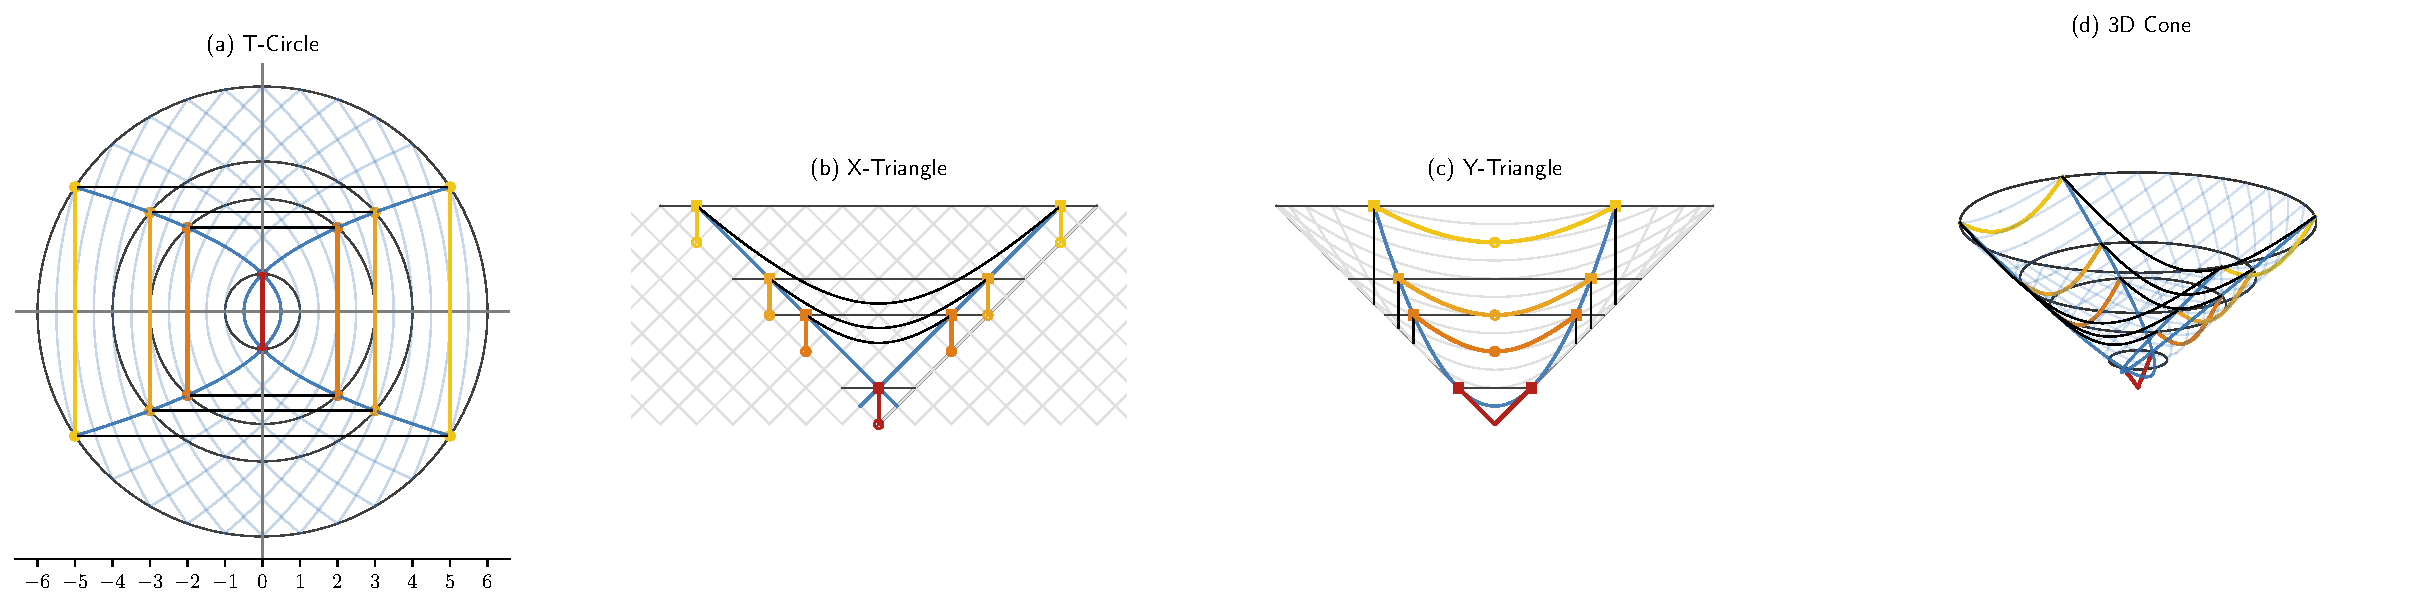
\includegraphics[width=\textwidth]{fig_totient_hyperbolas_4panel}
\caption{The four totient hyperbolas, four views of one object:
(a) down the $T$ axis, (b) down $Y$, (c) down $X$, (d) perspective.
For each unit $r\in\{1,5,7,11\}$ the colored arc is the Paper-A
hyperbolic section $X=(r-1)/2$ (yellow $r=11$ to red $r=1$, degenerate),
running from the open-circle vertex $((r-1)/2,0,(r-1)/2)$ to the
unit-shell squares $(\pm(r-1)/2,\pm\sqrt r,(r+1)/2)$ on the landing
circles $T=(r+1)/2$ (thin gray); black connectors join the shell points
at constant $Y=\sqrt r$.  The vertices $X\in\{0,2,3,5\}$ and the radii
$T\in\{1,3,4,6\}$ square to $QR(12)=\{0,1,4,9\}\bmod 12$, the two
bijections of Proposition~\ref{prop:bijection}.}
\label{fig:hyperbolas}
\end{figure}

\section{Scope}

The placement realizes the bijection; it does not define the group law
of $U(12)$, whose multiplication is prior arithmetic.  The content of
Proposition~\ref{prop:bijection} is exact finite arithmetic read off the
cone geometry, in the same spirit as Paper A's exact conic
classification.

\begin{remark}
The author views this double bridge --- the same four units read off
twice, once at the hyperbola vertices and once on the landing circles
--- as the geometric form of mod-$12$ uniqueness in the cone project:
the reason the number $12$, and not a neighboring integer, is the one
whose unit shell closes exactly onto its own quadratic residues.  It is
also the picture the project grew out of: the unit shell came first,
and the discriminant-$12$ program was built outward from it.
\end{remark}

\section*{Acknowledgment}
Large language model tools were used for machine verification, figure preparation, and drafting.

\begin{thebibliography}{9}
\bibitem{Ebert2026Table} J.~Ebert, \emph{The Cutting Plane: Every Line Through the Multiplication Table Is a Conic Section}, Preprint (2026).
\end{thebibliography}
\end{document}
